%!TEX root = ../../report.tex

\subsection{Inverse Design [NOT DONE]} % (fold)
\label{sub:inverse_design}


In \cite{Vanegas2009} it is presented a different solution from the others already presented.

It's described a framework that enables high level control of the modelling process. It ``provides a mechanism to interactively edit urban models". They apply inverse design to solve the problem of output control. From an existing model, the user can specify high level indicators that describe the desired output and the system change the underlying rules and parameters to get the result as close as possible to the desired.

As the Figure~\ref{fig:loop} shows, the user can change the ``low level" parameters and the ``high level" indicators to control the final output of the system.

\begin{figure}[htbp]
	\centering
	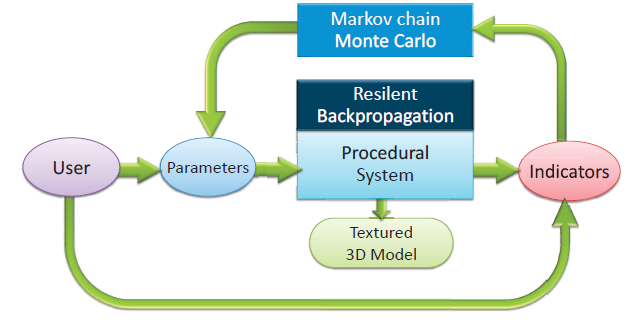
\includegraphics[width=0.95\textwidth]{img/Inverse_Design/TheLoop.PNG}
	\caption{System Pipeline \cite{Vanegas2009}}
	\label{fig:loop}
\end{figure}

This framework uses the indicators as a goal to optimize the parameters. To calculate the values for the parameters they used a version of Monte Carlo Markov Chains (or MCMC) and Resilient Back Propagation.


They implemented a urban procedural engine ``similar to previous city-level procedural modelling work". It was inspired by urban planners, that use the place types concept to represent coherent design patterns of buildings and streets. 


With this approach, the authors claim two main advantages, \emph{Abstraction} and \emph{Interactivity}. They argue that this solution allows urban planners and designers to work at a high level of abstraction, enabling users to manipulate place types, parameters and indicators to create the 3D model they want without wasting time with low level tasks as implementation of low level rules or parameter tuning.

At the same time this approach enables the users to interactively manipulate very complex indicator targets with a ``sophisticated enough" methodology to map target indicators to input low level parameters.


With their teilored version of MCMC and back-propagation they are able to support complex indicators ``enabling control beyond global shape, sush as by high-level semantics and indicators'', and by considering the procedural model as a black box there aren't any limitations to the used grammar.


% \subsubsection{Overview} % (fold)
% \label{ssub:overview}

% A system $P$ produces a geometry $G$ based on \emph{m} input parameter values $\Phi = \{\phi_1,\dots,\phi_m\}$ that is evaluated by an indicator measurement system $I$ which produces a set $\Gamma = \{\gamma_1,\dots,\gama_n\}$ of \emph{n} indicator values.


% % subsubsection overview (end)


% \subsubsection{Inverse Design} % (fold)
% \label{ssub:inverse_design}

% $\Gamma$ - Indicator Values

% $\Phi$ - Input Parameters

% $\Gamma*$ - Target Indicator Values

% $\Phi*$ - Target Parameter Values (specification is optional)


% % subsubsection inverse_design (end)


% \subsubsection{Urban Procedural Model} % (fold)
% \label{ssub:urban_procedural_model}



% subsubsection urban_procedural_model (end)


(\dots ?)

% subsection inverse_design (end)
